\documentclass[a4paper,12pt]{report}

\usepackage{alltt, fancyvrb, url}
\usepackage{graphicx}
\usepackage{subfigure}
\usepackage{wrapfig}
\usepackage{algorithmic}
\usepackage[utf8]{inputenc}
\usepackage{fontenc}
\usepackage{amsmath,stmaryrd,mathtools,algorithm}
\usepackage{amssymb}
\usepackage{float}
\usepackage{hyperref}
\usepackage{titlesec}

% Remove option to use English naming
\usepackage[italian]{cleveref}

% Questo commentalo se vuoi scrivere in inglese.
\usepackage[italian]{babel}

\title{Relazione per\\``DPG - Dope Party Game''}

\author{Davide Freddi\\Davide Picchiotti\\Miriana Ascenzo\\Riccardo Squarcialupi}
\date{\today}

\begin{document}

	\maketitle

	\tableofcontents

	\chapter{Analisi}
	\section{Requisiti}
	Il software DPG - Dope Party Game consiste in un gioco a turni, in cui l'obiettivo è far arrivare il proprio personaggio in fondo a un tabellone, costituito da uno o più percorsi formati da caselle.
	%
	Alla fine di ogni turno, vengono fatti fare dei minigiochi a ogni giocatore.

	\subsubsection{Requisiti funzionali}
	\begin{itemize}
		\item il software deve presentare un menu principale all'avvio, che permetta di avviare il gioco con diverse opzioni, quali numero di giocatori e numero di CPU
		\item il gioco viene giocato da più giocatori nello stesso computer, prendendo il controllo durante il proprio turno
		\item ai giocatori viene fatto tirare un dado, che determina quanti passi vengono fatti all'interno del tabellone
		\item esistono diversi tipi di celle, che possono causare diversi eventi quando un personaggio ci finisce sopra
		\item alla fine di ogni turno viene scelto casualmente un minigioco da far fare a tutti i giocatori, e in base alla posizione nella classifica dei punteggi vengono assegnati dadi migliori o peggiori
		\item ogni CPU ha una difficoltà, che determina i suoi punteggi nei minigiochi
		\item i minigiochi possibili sono:
		\begin{itemize}
			\item ballgame - bisogna far arrivare una palla in fondo a un percorso il prima possibile, e alcuni muri fanno tornare all'inizio se colpiti
			\item punchygame - bisogna colpire piu' sacchi possibili, mirando nella direzione giusta
			\item molegame - bisogna colpire più talpe possibili entro lo scadere del tempo
			\item jumpgame - bisogna arrivare più in alto possibile rimbalzando su delle piattaforme
		\end{itemize}
	\end{itemize}

	\section{Analisi e modello del dominio}

	Il programma partirà da un menu, che al momento opportuno avvierà il gioco.
	%
	All'avvio del gioco il menu notificherà il ciclo di gioco (GameCycle), che gestirà una serie di personaggi (Character).
	%
	I personaggi si muovono all'interno di una griglia (Grid) composta da caselle (Cell), e possono essere controllati o da un giocatore, o da una cpu (CPU), gestita del ciclo di gioco.
	%
	Alla fine del turno il gamecycle avvierà dei minigiochi (Minigame), che ritorneranno un certo punteggio intero.
	%
	Le difficlotà primarie potrebbero essere le seguenti:
	\begin{itemize}
		\item gestire le cpu in maniera intelligente, evitando di complicare eccessivamente il codice
		\item generare una griglia senza impostarne tutti i dettagli manualmente dal codice
		\item generare diverse configurazioni di griglie con un codice flessibile
		\item individuare una struttura di codice basilare e comune per i minigiochi
		\item gestire le collisioni e la fisica nei minigiochi che lo richiedono
	\end{itemize}

	\begin{figure}[!t]
		\centering{}
		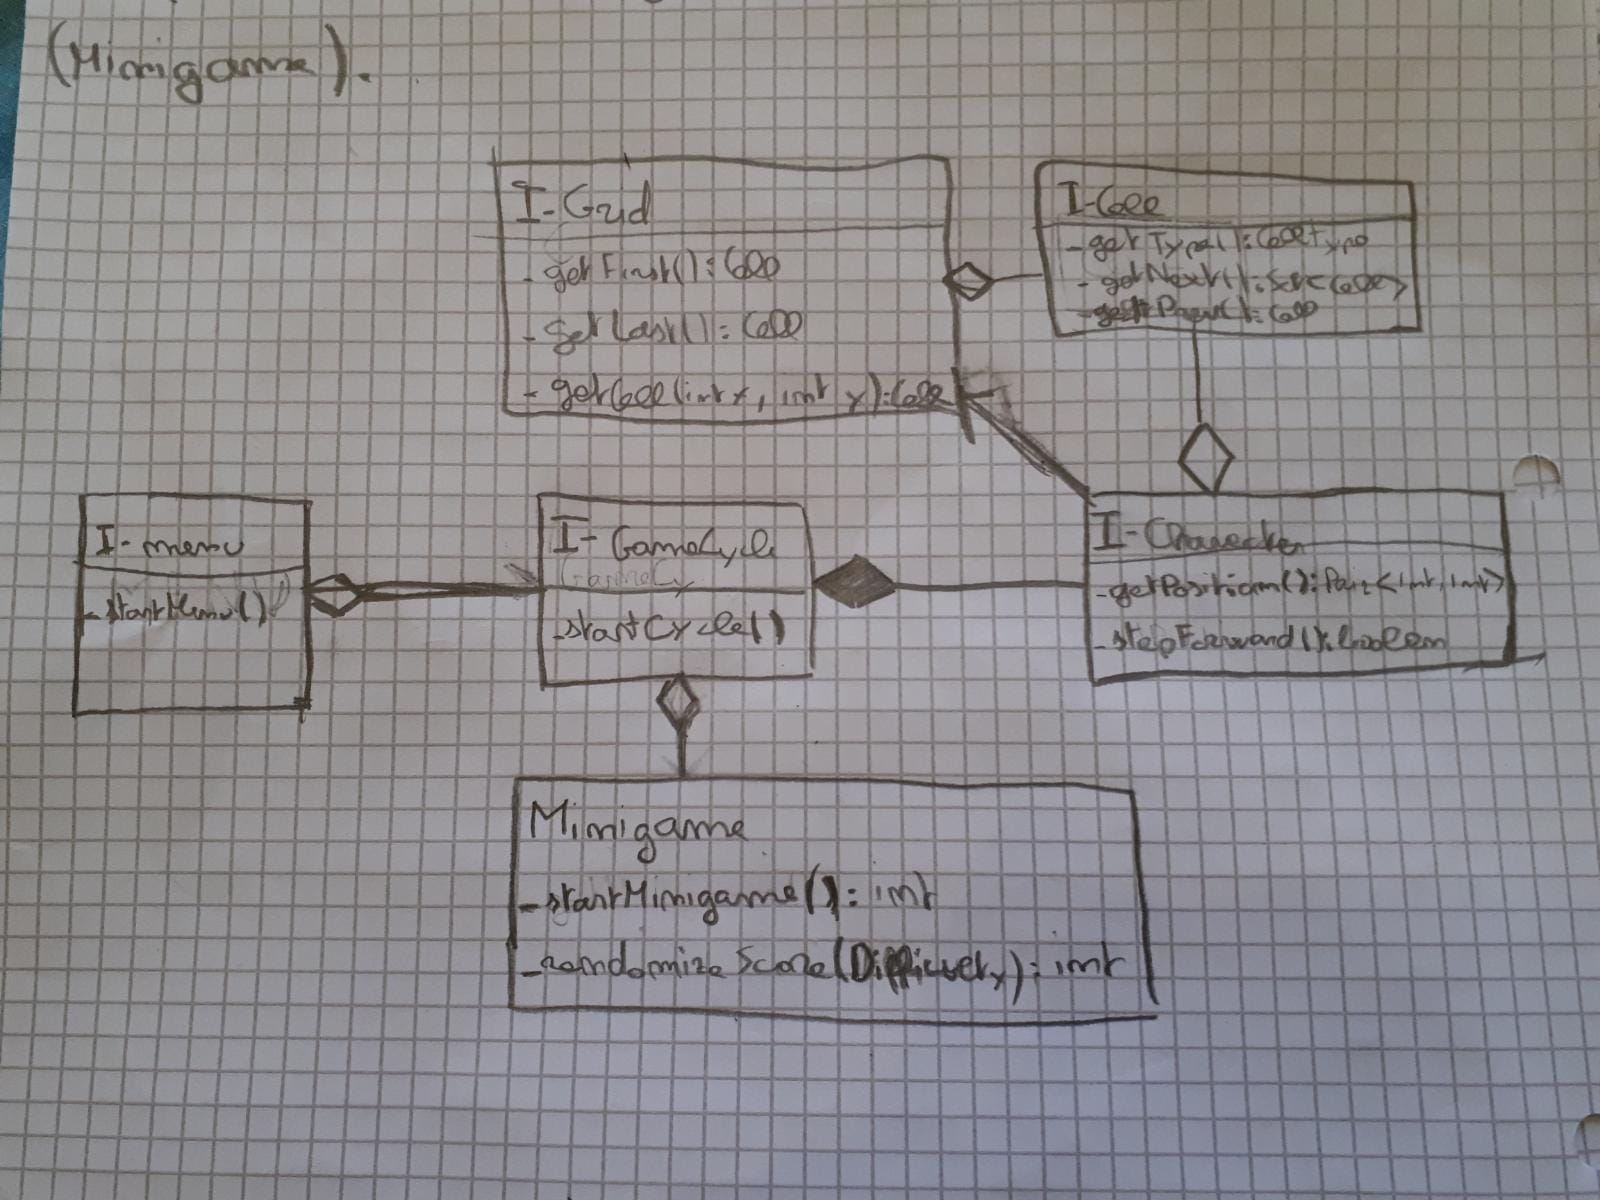
\includegraphics[width=150mm]{images/domain.jpeg}
		\caption{Schema UML dell'analisi del problema, con rappresentate le entità principali ed i rapporti fra loro}
		\label{img:analysis}
	\end{figure}

	\chapter{Design}

	\section{Architettura}

	L'architettura del software segue il pattern architetturale MVC.
	%
	Il menu è composto da una View (MenuView), e un Controller (MenuController) che ne cattura gli eventi e ne comanda le modifiche.
	%
	Quando il gioco viene avviato il Controller del menu avvia il ciclo di gioco (GameCycle).
	%
	Il ciclo di gioco avvia un nuovo thread in background che si occupa di gestire una serie di personaggi e le varie CPU, gestire la sequenza dei turni nel gioco, e aggiornare la View della griglia (Gridview) quando necessario.
	%
	Il Character rappresenta un personaggio in grado di tirare il proprio dado e spostarsi all'interno della griglia (Grid).
	%
	La CPU si occupa invece di fare le decisioni che spetterebbero normalmente al giocatore, come scegliere il percorso da fare in un bivio.
	%
	Il Character tiene traccia della propria posizione tramite un riferimento alla casella (Cell) su cui si trova.
	%
	La casella contiene delle coordinate e il riferimento alle caselle successive e precedenti nel tabellone.
	%
	La griglia gestisce le caselle, e permette di ottenere la prima e l'ultima casella del percorso, o una certa casella date delle coordinate.
	%
	Minigame si occupa di eseuire il minigioco, o ottenere un punteggio per una CPU in base alla sua difficoltà.
	%
	Ogni minigioco avrà a sua volta delle ulteriori interfacce di View, Controller e Model.

	\begin{figure}[!t]
		\centering{}
		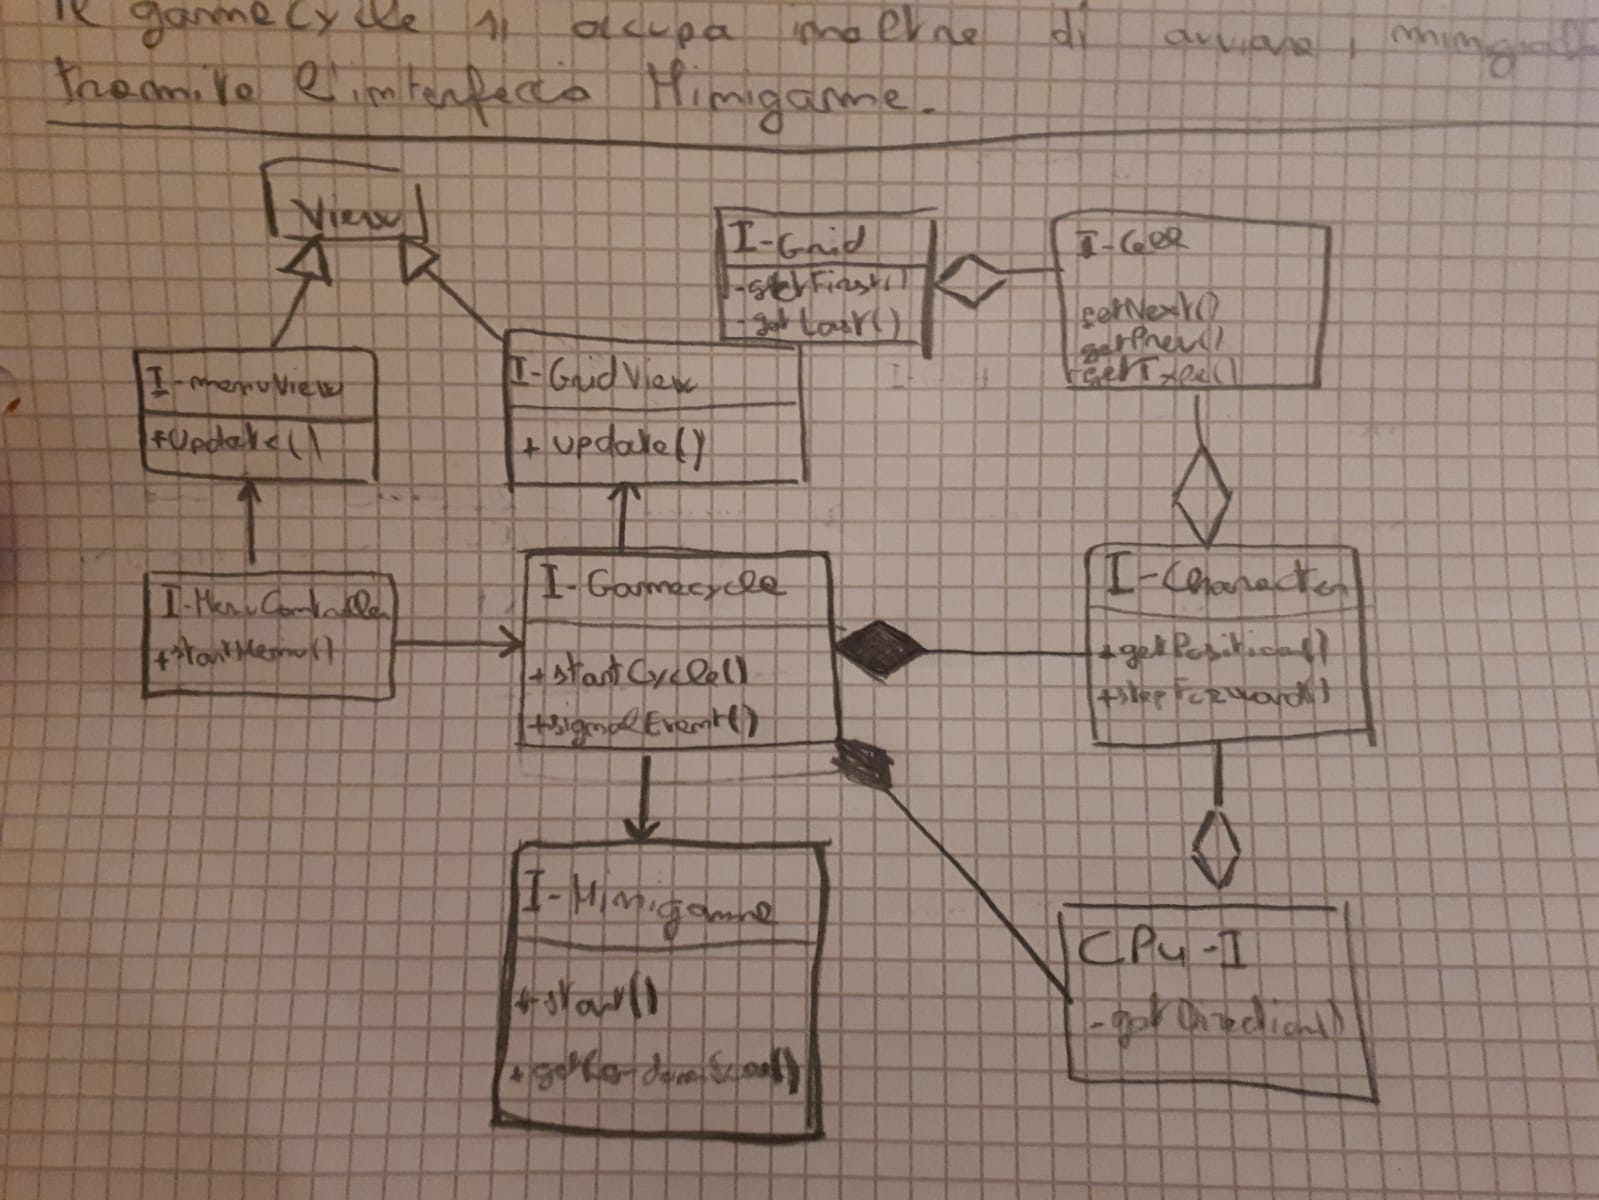
\includegraphics[width=\textwidth]{images/arch.jpeg}
		\caption{Schema UML architetturale di DPG. View, GridView e MenuView sono interfacce di view, Gamecycle e Minigame sono interfacce di controller, mentre Grid, Cell e Character sono interfacce di modello.}
		\label{img:goodarch}
	\end{figure}
	%
	\section{Design Dettagliato}
	%
	\subsection{Design dettagliato Davide Freddi}
	Design dettagliato davide freddi
	%
	\subsection{Design dettagliato Davide Picchiotti}
	\subsubsection{Modellazione dei giocatori}
	In questa sezione si tratterà il design dei giocatori all'interno del modello.\newline
	\newline
	Ogni giocatore (umano e non) viene rappresentato tramite l'interfaccia Character.
	Questo espone metodi per controllare tutti gli aspetti relativi a un dato giocatore durante la partita:\begin{itemize}
																											   \item movimento step-by-step nella griglia
																											   \item lancio di dado
																											   \item salvataggio di valori importanti durante la partita (turno, posizione, punteggio dei minigiochi ecc.)
	\end{itemize}
	%
	L'avanzamento del giocatore con gli appositi metodi avviene step-by-step, ovvero si muoverà di una
	casella per ogni chiamata; è stata presa questa direzione di design per fare in modo che durante
	uno stesso lancio di dado, tra una casella e l'altra, si potessero scatenare eventi sul giocatore
	dovuti dal tipo di casella attraversata.\newline
	%
	//immagine uml character\newline
	\caption{Schema UML delle classi relative a Character}
	%
	Per fare in modo che nella partita siano presenti giocatori non umani (CPU) è necessario servirsi
	dell'interfaccia Cpu.\newline
	Le sue implementazioni dovranno contenere un Character in modo da poter "prendere le decisioni" in vece del giocatore, come la direzione da prendere a un bivio.\newline
	Inoltre ogni Cpu avrà assegnata una difficoltà (enum Difficulty) che al momento stabilisce unicamente il punteggio che otterrà nei minigiochi.\newline
	In questo modo è possibile creare nuovi tipi di Cpu con diversi comportamenti in maniera disaccoppiata.
	%
	//immagine uml cpu\newline
	\caption{Schema UML delle classi relative a Cpu}

	\subsubsection{Struttura base dei minigiochi}
	In questa sezione si tratterà delle classi e interfaccie che stanno alla base di tutti i minigiochi del progetto.\newline
	\newline
	I minigiochi sono stati trattati come piccoli progetti a sé stanti da integrare poi nel gioco completo, con il semplice requisito che ognuno di essi ritorni un punteggio intero.\newline
	%
	Le classi e le interfaccie presentate sono state pensate con lo scopo di avere un buona struttura MVC per ogni minigioco e allo stesso tempo aver un entry-point definito per l'avvio e il settaggio di qualunque minigioco. L'unica parte architetturale che non viene definita da questa struttura è il Model di ognuno, poiché considerato troppo specifico in base al tipo di minigioco che si intende realizzare.\newline
	%
	//immagine uml minigiochi\newline
	\caption{Schema UML delle classi relative a Cpu}
	%
	Per far sì che la routine di avvio e settaggio del minigioco fosse uguale per ognuno si è adottata la strategia delle classi astratte con Template Method.
	Nello specifico AbstractMinigameView ha il metodo template createScene() per la creazione della Scene di JavaFX e AbstractMinigame ha i metodi template getMaxScore (per il calcolo del punteggio), createGameCycle() (per la creazione del ciclo di gioco) e createView() (per la creazione della View).\newline
	Inoltre l'interfaccia Minigame ha l'unico metodo start() che fornisce un entry-point univoco per qualunque minigioco implementato in maniera corretta.\newline
	\newline
	Il punto debole di questa soluzione è che le classi astratte proposte andranno modificate o sostitutite se si sceglie di utilizzare un componente grafico diverso da JavaFX. Mettendo sulla bilancia questo aspetto negativo con quello positivo di poter "generalizzare" il comportamento del minigioco alle fondamenta, è stato considerata comunque una soluzione valida per la quantità esigua di modifiche che richiederebbe la sostituzione del componente grafico.

	\subsubsection{Punchy Minigame}
	In questa sezione verrà trattato nel dettaglio il design del minigioco Punchy.\newline
	\newline
	Per il design di questo minigioco ci si è per lo più limitati a implementare le opportune interfacce e a estendere le classi astratte. Sono state create interfacce aggiuntive per la gestione della View (PunchyminigameView) e del Model (World).
	\newline
	//uml punchygame overview\newline
	\newline
	In generale, l'interfaccia PunchygameView permette di gestire tutti gli aspetti della View che rispecchiano il Model del gioco, ma la classe che la implementa necessita anche l'estensione di AbstractMinigameView per poter settare e chiudere la View stessa. L'interfaccia consente comunque di scorporare la View e di cambiare in maniera agevole il componente grafico.\newline
	Inoltre è stato utilizzato il pattern Observer per la gestione degli input dell'utente: la View (PunchygameView) è il componente osservato, mentre l'osservatore sarà nel Controller (PunchygameCycle) e otterrà gli input tramite InputObserver.\newline
	Gli input da propagare verso il Controller sono modellati con l'interfaccia Input, che con pattern Strategy ci permette di cambiare a seconda delle esigenze gli input da passare a InputObserver. Essendo necessari solo due comandi per rappresentare il pugno a destra e a sinistra (molto simili tra loro) si è optato per una classe astratta che implementa Input e fa uso del pattern Template Method per farsi fornire dai suoi sottotipi la Direction del pugno.
	Il metodo template in questione è getPunchDirection() in AbstractPunch.
	\newline
	//uml punchygame view\newline
	//uml punchygame input\newline
	\newline
	%
	La parte di Model è molto semplice, in quanto presenta la classe World come unico entry-point del model, la cui implementazione userà al suo interno i vari componenti Boxer, Timer, Score. La componente dei sacchi da boxe del gioco non ha necessitato di una classe specializzata, poiché modellabile con una semplice lista all'interno di WorldImpl.\newline
	\newline
	//uml punchygame model\newline
	\newline
	%
	La parte di Controller è costituita dal ciclo di gioco, ci si limita quindi a implementare l'interfaccia
	MinigameCycle. Naturalmente è necessario avere un InputObserver all'interno del Controller e si è optato per l'implentazione di esso direttamente nella classe PunchygameCycleImpl.
	\newline
	//uml punchygame controller\newline
	\newline
	%
	\subsection{Design dettagliato Miriana Ascenzo}

In modello, una classe GridInitializer si occupa della creazione di una Grid, ovvero un Tabellone di Gioco, partendo da un GridType.
%
GridInitializer cerca, in base al tipo di Griglia passatogli, un file json corrispondente: tale file viene letto tramite l'uso della libreria Jackson.
%
La classe è stata sviluppata quindi in modo tale da rendere automatica la creazione di una grid diverse in base al json, seguendo sempre lo stesso procedimento.
%
I dati vengono letti raccolti dal json Cella per Cella, tramite la classe CellParser.
%
Vengono quindi create diverse Cell, che compongono una Grid.

\begin{figure}[h]
	\centering{}
	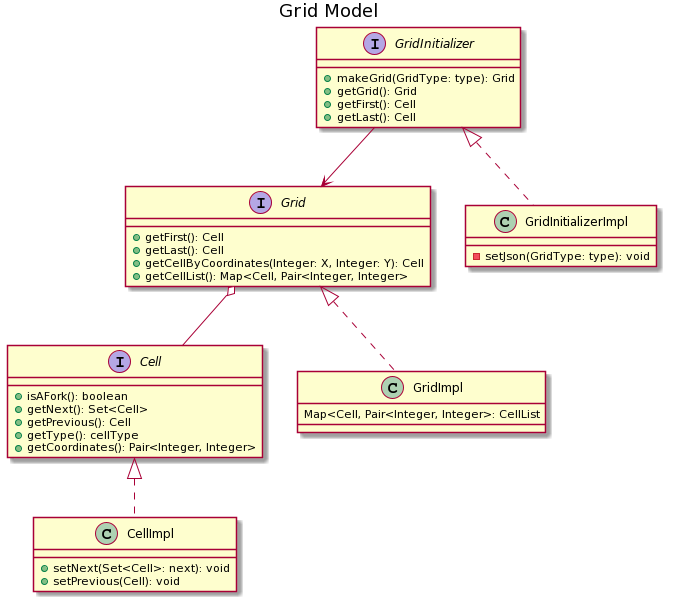
\includegraphics[width=\textwidth]{images/miriana/grid_model.png}
	\caption{Schema UML della generazione di una Grid e della sua struttura.}
	\label{img:gridmodel}
\end{figure}

In controller, abbiamo una classe GridGenerator: tramite il suo unico metodo generate(), vengono creati prima una Grid, e poi una GridView basata su tale Grid.
%
Una Grid viene creata a partire dagli elementi che gli vengono forniti: GridGenerator prende per costruttore una GridType (enum di possibili griglie) e tramite essa cerca nelle resources un file Json corrispondente.
%
GridGenerator riceve inoltre un GameCycle: questo verrà passato a GridView affinchè la view generi il suo GridObserver.

\begin{figure}[h]
\centering{}
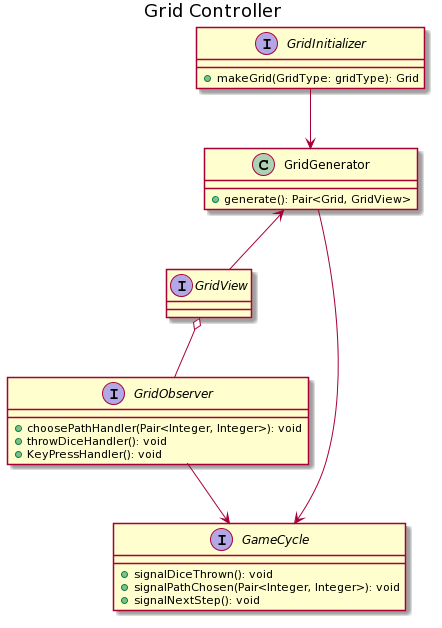
\includegraphics[width=\textwidth]{images/miriana/grid_controller.png}
\caption{Schema UML del controller di Grid e di come interagisce con GameCycle}
\label{img:gridcontroller}
\end{figure}

La View della Griglia estende da View, e viene in seguito implementata affinchè generi i nodi necessari.
%
La generazione di alcuni nodi ripetuti viene gestita in una classe ViewNodesFactory: essa genera le Celle in base alla posizione, le linee che collegano tali Celle, e i player.
%
La View può essere sostituita in blocco grazie al modello MVC: essa non riceve mai elementi di modello, solo riferimenti.

\begin{figure}[h]
	\centering{}
	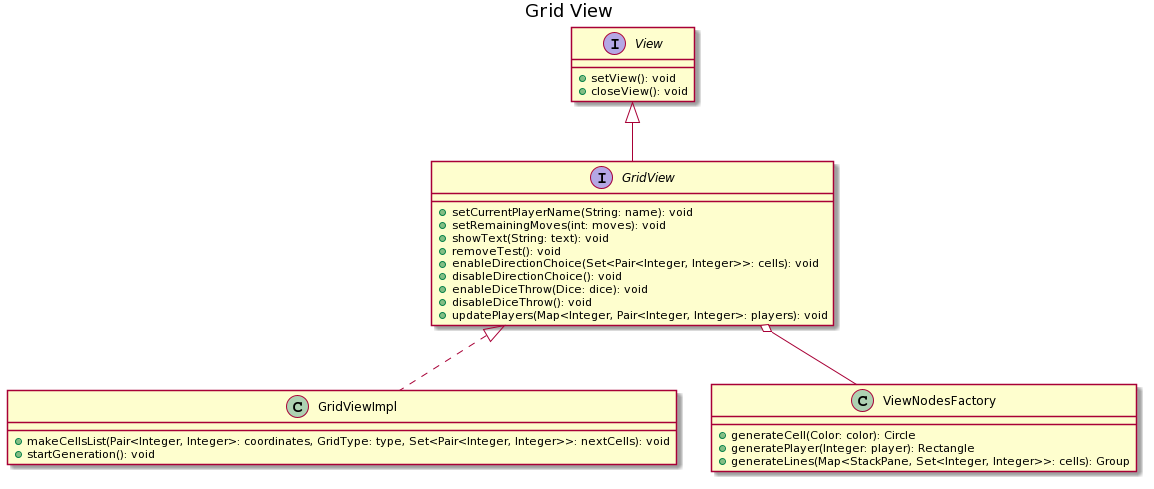
\includegraphics[width=\textwidth]{images/miriana/grid_view.png}
	\caption{Schema UML della View della Grid}
	\label{img:gridview}
\end{figure}

Gli elementi di GridView che ricevono input dall’esterno, ad esempio i bottoni, hanno il ruolo di informare il gameCycle di quale azione è stata intrapresa da chi sta usando il software.
%
Per questo viene generato GridObserver, una classe di pattern Observer.
%
La classe GridObserver ha per Observable GridViewImpl: Se un determinato bottone viene premuto, o una determinata key sulla tastiera viene premuta, viene inviato un segnale al GameCycle.

\begin{figure}[h]
\centering{}
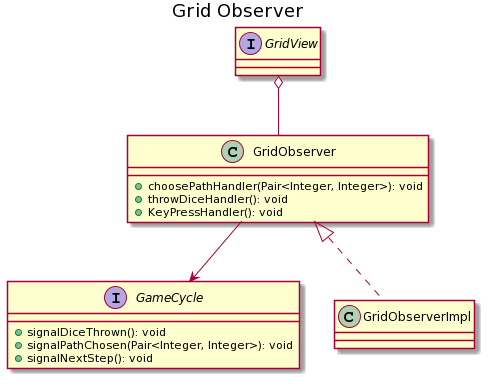
\includegraphics[width=\textwidth]{images/miriana/grid_observer.png}
\caption{Schema UML dell'interazione fra GridView e GameCycle. Segue il pattern Observer.}
\label{img:gridobserver}
\end{figure}

I nodi di GridViewImpl vengono aggiornati in runtime ogni volta che gli elementi all’interno del software, quali players, dices, scritte da rappresentare, vengono modificati dal controller (ovvero il gameCycle).
%
Per aggiornare i nodi correttamente in runtime, esiste una classe GridViewPlat: quest'ultima implementa GridView, e riceve da GridGenerator una GridViewImpl.
%
GridViewPlat chiama i metodi di GridViewImpl nel thread dell’applicazione JavaFX.
%
Questo avviene tramite l’uso di Platform.runLater.
%
Quello che succede in GridGenerator è quindi: una GridViewImpl viene creata a partire da una Grid, e in seguito, a partire da GridViewImpl, viene creata una GridViewPlat, responsabile dell’aggiornamento della View nel thread dell’applicazione JavaFX.
%
Abbiamo un pattern Proxy, per cui gameCycle accede a GridViewPlat (proxy), il quale contiene GridViewImpl (real target), per aggiornare la View.

\begin{figure}[h]
\centering{}
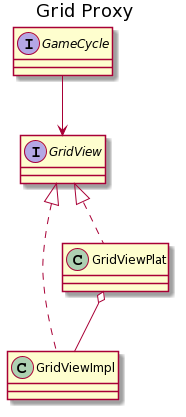
\includegraphics[width=\textwidth]{images/miriana/grid_proxy.png}
\caption{Schema UML di come GameCycle accede a GridViewImpl. Segue il pattern Proxy.}
\label{img:gridmediator}
\end{figure}

	\subsection{Design dettagliato Riccardo Squarcialupi}
	Design dettagliato Riccardo Squarcialupi

	\chapter{Sviluppo}
	\section{Testing automatizzato}

	\subsection{Davide Freddi}
	\subsection{Davide Picchiotti}
	\subsection{Miriana Ascenzo}

	È stata sottoposta a test automatici la creazione di una Grid a partire da uno specifico gridType.
	%
	Vengono fatti dei test sul giusto collegamento fra Celle e sul giusto contenimento o meno di alcune celle nella Grid creata.
	%
	Per la View sono stati eseguiti dei test automatici facendo uso della libreria TestFX; in particolare sono stati testati il corretto aggiornamento del Label principale nella view (dove appaiono le scritte del tipo “start game”, “dice result”),
	%
	il corretto aggiornamento della posizione dei player all'interno della mappa, e la possibilità di cliccare o meno il button per tirare il dado in base a se il tiro è abilitato o disabilitato.


	\subsection{Riccardo Squarcialupi}

	\section{Metodologia di lavoro}

	Descrizione separazione?

	\subsection{Sezione Davide Freddi}
	\subsection{Sezione Davide Picchiotti}
	\subsection{Sezione Miriana Ascenzo}

	Il ruolo nel gruppo è stato quello di creare strutture dati per le Celle e la Griglia del gioco, la creazione delle stesse a partire da un json, e la creazione di una View che rappresentasse la griglia creata e che si aggiornasse in tempo reale in base ai cambiamenti dettati dal controller.
	%
	Un problema presentatosi durante la fase d’integrazione, è stato la dimenticanza in fase di design di un metodo “getPrevious” in Cell; il metodo serve per poter implementare la funzionalità “StepBackwards”, ovvero la possibilità di tornare indietro nella griglia.

	\subsection{Sezione Riccardo Squarcialupi}


	\section{Note di sviluppo}

	\subsection{Davide Freddi}
	\subsection{Davide Picchiotti}
	\subsection{Miriana Ascenzo}

	Feature avanzate usate:
	\begin{itemize}
		\item lambda
		\item stream
		\item librerie esterne (Jackson, JavaFX, TestFX, Mockito)
	\end {itemize}
	La libreria Jackson permette di leggere il contenuto di un file json e di tradurlo tramite un mapper e un parser.
	%
	La classe GridInitializer fa uso di un’altra classe CellParser, con la quale, tramite il mapper, vengono raccolti i dati Cella per Cella e inseriti nella struttura dati.
	%
	La classe TestFX permette di eseguire test sulla GUI.
	%
	La classe Mockito permette, in fase di test, di creare classi Mock a partire da interfacce esistenti (simulano il comportamento di classi che implementano tali interfacce).

	\subsection{Riccardo Squarcialupi}

	\chapter{Commenti finali}

	\section{Davide Freddi}
	\section{Davide Picchiotti}
	\section{Miriana Ascenzo}

	Punti di forza:
	%
	Il lavoro è stato svolto in maniera abbastanza lineare, realizzando in ordine le diverse fasi del progetto.
	%
	Le classi di generazione del Tabellone di Gioco e di View sono state automatizzate al meglio delle capacità, risultando in una view facilmente sostituibile.
	Punti di debolezza:
	%
	Sono stati fatti errori di distrazione, il che ha richiesto dover tornare indietro nel codice più volte pe trovare tali errori e correggerli.


	\section{Riccardo Squarcialupi}

	\appendix
	\chapter{Guida utente}

	Spiegazione comandi e utilizzo del gioco

All'avvio del gioco compare un menù: premere start avvia un game in impostazioni standard (2 giocatori, di cui uno è una CPU).
%
Se si vuole modificare il numero di giocatori e/o il numero di CPU, premere Options ed inserire le preferenze.
%
Una volta premuto start il game inizia con i giocatori sulla casella start.
%
Da qui bisogna seguire le istruzioni che vengono dettate nel riquadro bianco più in alto:
\begin {itemize}
	\item quando appare l'istruzione "continue..", premere invio per proseguire
	\item quando appare l'istruzione "Throw the Dice!", il bottone dado sottostante verrà abilitato: premere il bottone per tirare il dado
	\item quando appare l'istruzione "choose the direction on the map", due bottoni verrano abilitati: premere il bottone corrispondente alla casella che si vuole raggiungere
\end {itemize}
Ogni turno finisce con un minigioco: ottenere più punti possibili per vincere dadi migliori da tirare.
Istruzioni minigiochi:
\begin {itemize}
	\item ballgame: premere le frecce direzionali per comandare la palla rossa. Raggiungere il traguardo evitando i muri rossi nel tempo limite(punteggio basato sul tempo impiegato).
	\item punchygame: premere le frecce direzioni destra e sinistra per colpire i sacchi da boxe rossi. Colpirne il maggior numero nel tempo limite (punteggio basato sul numero di sacchi colpiti).
	\item jumpgame: premere le frecce direzionali per comandare il quadratino. Saltare più piattaforme possibili senza cadere o toccare i bordi laterali della finestra (punteggio basato sul numero di piattaforme saltate).
	\item molegame: premere start per avviare il minigioco: cliccare su più talpe possibili nel tempo limite (punteggio basato sul numero di talpe cliccate).
\end {itemize}
Il gioco finisce quando un giocatore raggiunge l'ultima casella del Tabellone, vincendo il game.


\bibliographystyle{abbrv}
\bibliography{template}

\end{document}
